%# -*- coding: utf-8-unix -*-
% !TEX program = xelatex
% !TEX root = ../thesis.tex
% !TEX encoding = UTF-8 Unicode
%%==================================================
%% chapter01.tex for SJTU Master Thesis
%%==================================================


%10.5 pages, just ~28 rows in one page, not mentioning single column.
\chapter{引言}
\label{chap:intro}

%什么叫理解,
%注意:几句话扯一下就可以了(4句话)
%“基于知识库的自然语言关系语义建模”

本文主要的研究对象是自然语言中的单词、短语以及句子。
%自然语言理解的主要难题在于,字面形式的多样性,
%不同写法,相同含义
%多种不同的表示形式,给机器理解提出了挑战。
%人类理解自然语言句子的时候,会最关注两类信息,
为了使机器可以像人类一样,理解一个句子背后的含义,而不是仅仅停留在识别字面上的不同词汇,
我们需要让机器挖掘出句子中的两类信息,
即句子里的实体(人物、地点、组织、事件等),
以及实体之间的关系。
考虑到自然语言描述方式的多样性,
我们需要使用标准化的数据库作为语义理解的载体,
其包含自然界中所有已知的实体,以及它们之间存在的关系,
这样的结构化数据库被称为知识库。
本文研究的问题,就是将自然语言中的实体、关系以及句子的语义,映射到知识库的过程。
%may add one more sentence here.

\section{研究背景}
\label{sec:intro-background}

% %给直观的例子,甚至越早越好
% 
% 自然语言理解是人工智能(AI)的一个重要分支。
% 早在1950年,英国科学家阿兰$\cdot$图灵就提出了著名的思想实验``图灵测试''~\cite{},
% 即让机器作为被测试者,仅通过文本与人类测试者对话,并说服人类自己是人而不是机器。
% 若人工智能通过了图灵测试,则意味着其语言理解的能力已达到接近人类的水平。
% 
% %然而,实现人类水准的语言理解能力难度巨大,目前通过图灵测试的AI大多靠避而不答,而不是正面回答问题\cite{warwick2016ca}。
% %然而,目前AI的语言理解能力远未达到人类水平,
% 然而,实现该水准的人工智能难度巨大,这源于自然语言理解所具有的复杂性。
% 
% 这种复杂性首先体现在自然语言所能描述的信息量大。
% 随着互联网的发展,越来越多人类知识以网页的形式进行存储。
% 截至2018年6月,Google搜索引擎已索引大约470亿个网页
% \footnote{\url{http://www.worldwidewebsize.com/}},
% 考虑到大量未被索引的网页以及未被电子归档的书籍资料,
% 人类所拥有的知识远不止统计数据所显示的规模。
% 并且随着新事件的发生,新的知识也还在不断涌入。
% 如何管理大量知识成为了人工智能的难点。%这句需要修改
% %考虑引用warwick的
% 另一方面,自然语言本身的描述具有多样性,
% 同样的语义可以对应不同字面形式的句子,
% 而同样的词汇在不同的语境下,也可以对应不同的语义。
% 这样的语句复述和一词多义在自然语言中非常常见,
% 也是自然语言理解面临的主要难点。
% %多义性和同义性
% %感觉应该多说一些东西,但现在还不确定怎么说。先写后面的吧
% 
% 
% %整理知识的两个方向:
% %为了解决。。。的问题
% %整理知识的两个方向的努力:OpenIE和KB
% 
% %途径1,将非结构化信息整理
% 在知识整理方面,%为了从非结构化文本中提取知识,
% 信息抽取技术(Information Extraction)的任务是
% 从句子中提取出特定类型的实体(Entity)以及实体之间的关系(Relation),
% 组成实体关系三元组$(Arg_1, Relation, Arg_2)$,
% 其中$Arg_{1,2}$分别代表关系的头实体和尾实体。
% 以句子``Mozart was born in Salzburg, but moved to Vienna in 1781''为例,
% 其中包含了三元组(Mozart, was born in, Salzburg)以及(Mozart, moved to, Vienna)。
% 对比传统传统命名实体识别任务\cite{}中的人名、地名、组织名,
% 类型更加广泛,电影、事件、等等blabla的类别。
% 早期的信息抽取主要针对特定领域的文本数据,
% 而近年来提出的开放式信息抽取(Open Information Extraction),
% 目的就是在不限定领域的海量文本中提取实体和关系。
% 
% % 典型论文:TR,RV-PATTY,再搞个新的
% % 
% % 而TextRunner系统\cite{}
% % 
% % 理解句子内的信息
% % 对非结构化的纯文本进行信息提取
% % 并不限制于某一特殊领域
% % 称为开放式信息提取(Open Information Extraction)。
% % 目标:非结构化到半结构化
% % 识别句子中的实体
% % 
% % 
% % TextRunner,ReVerb,OLLIE。。。。PATTY,NELL
% % 稍微讲一下方法的演变
% % 
% % 典型:ReVerb,PATTY:(主, 谓, 宾)三元组,
% % 主语,宾语是。。。。实体 并不局限于语法分析里的nsubj,dobj
% % 谓语:反正都是字符串
% % 
% % 实体关系三元组(Arg1, Relation, Arg2)
% % 
% % 
% % 
% % 知识的存储:对于非结构化,OpenIE
% % 开放信息抽取:非结构化到半结构化
% % 基本的主谓宾关系(简单的二元关系,以及复杂的多元关系出现在一个句子里)
% % 围绕自然界的实体相关的知识
% % 维基百科,社区构建,标准,量大
% % 半结构化
% % 
% % 斜体:知识库里的实体和关系,引号:字符串形式
% 
% %================%
% 
% 
% % %途径2:弄出知识库,作为知识的标准化载体
% % %弄一个FB的图,好看一点的
% % 通过社区进行人工构建的知识库,主要包括Wiki,DBP,Freebase,Google KnowledgeGraph
% % 结构化:讲一讲Ontology,Taxonomy这些玩意儿(重点讲)还有RDF
% % 
% % %注意联系:KB是我们的重点,但是结构上,OpenIE的SPO和KB里的<e1, p, e2>具有相似的性质。
% % %只不过OpenIE还没有被link而已。
% % 
% % 
% % 
% % %为什么要做上面这些努力:都是为理解自然语言做铺垫
% % %理解之后能干什么:阅读理解、对话机器人、自动问答、搜索引擎、等等场景。
% % %以搜索引擎为例子,传统的方式:TF-IDF(Bag-Of-Word)
% % %词向量,懂得什么是相似的词汇
% % %继续升级:语义理解,真正直接的理解意思,涉及到推理
% % %知识从哪来:KB啊,所以需要理解,问的是什么,以及关系是什么。
% % %真实例子:Google Search,
% % %由此引出中心问题。
% % 
% % 
% % 自然语言的理解
% % 为啥要做这些事情:因为要理解啊
% % 啥叫理解,搜索引擎是不是理解,简单的匹配是不是理解
% % 
% % 从直接匹配,到模糊匹配,到embedding,再到语义理解(截图)(不具体理解关系,是没法得到正确答案的)
% % 
% % 难度主要在哪里?东西很多啊,还要用好上下文啊,还有可解释性的问题
% % 
% % 可以展开聊一下可解释性的意义。
% % 
% % 知识库提供了天然的载体,机器可理解以及人类可读,可解释。
% % 因此论文关心的是,以知识库作为载体,将自然语言中的关系进行映射的过程。
% % 对应实体和谓语关系,会有不同的针对性研究。
% 
% 
% ================以上皆为无用嘴炮==================

%知识爆炸时代:
%信息量大,存储跟上,多大的数据,还不是人类的所有知识
人类的进化总是伴随着知识的不断积累。
传统的知识存储媒介为纸质书籍,
随着互联网的发展以及分布式存储系统的成熟,
越来越多人类知识以电子文档的形式进行存储。
截至2018年6月,Google搜索引擎已索引大约470亿个网页\footnote{\url{http://www.worldwidewebsize.com/}},
考虑到大量未被索引的网页以及未被电子归档的书籍资料,
人类所拥有的知识远不止统计数据所显示的规模。
并且随着新事件的发生,新的知识也还在不断涌入。
%人工智能场景:
身处信息化时代,人类和计算机的交互变得频繁,且交互方式呈现多样化。
而在这其中,自然语言一直是最重要的交互方式,
主要体现为文本和语音的形式,与人类之间的正常交流最为接近。
人工智能成为当今科研的热门方向,
由于计算机已经拥有海量的非结构化文本数据,
因此人类期望智能化的机器能够感知并掌握人类的知识,
从而更好地与人类进行自然语言交互。
科幻电影中经常安排了这样的机器人角色:
回答人类的提问,分析人类的情感,进行持续的聊天对话等等。
这些诉求支撑了自然语言处理领域的蓬勃发展。


%NLP一直是重要分支:
自然语言理解是人工智能的一个重要分支。
为了衡量机器在自然语言上的智能化水平,
早在1950年,英国科学家阿兰$\cdot$图灵就提出了著名的思想实验``{图灵测试}'' ,
%~\cite{},Computing machinery and intelligence
即让机器作为被测试者,仅通过文本与人类测试者对话,并说服人类自己是人而不是机器。
若机器通过了图灵测试,则意味着其智能化已达到接近人类的水平。
图灵测试属于开放领域的通用对话场景,
目前人工智能水平还远远不能达到这样的高度,
通过含糊其辞的策略进行对话可以做到欺骗人类测试者,
但这并非真正理解对话含义。
%极少数声称通过测试的AI\cite{warwick2016can}也主要以含糊其辞的策略对话,
%试图欺骗人类测试者,而并非真正理解对话含义。

%对于机器而言,自然语言就是一串符号的有序排列,之所以难以从中理解语义
之所以机器难以理解人类的语言,是因为自然语言本身具有很高的复杂性,
主要体现为两个方面。
一方面,自然语言中的不同词汇和语义之间不具有一对一关系。
人类语言并非遵循某种确定的规则产生,而是随着时间在不停演变,
例如``{苹果}'' 一词原本仅指代一种水果,
而苹果公司的出现,使得自然语言文本中的``{苹果}'' 有了明显的歧义。
可见,词汇和语义的对应来自约定俗成,并不需要满足严谨的区分度。
这使得同义词和一词多义成为了自然语言中的普遍现象。
另一方面,词汇的排列顺序也在影响着语义。
自然语言中存在着层次关系,多个词汇组成短语,多个短语组成句子等等。
组合而成的语义并不等于各个部分的简单叠加,
例如``{深度学习}'' 与``{学习深度}'' 两个短语具有较大的语义差别。
%若机器不能很好的了解结构化,就会出现类似于看得懂每个字,却看不懂整句话。

%确实难,涉及到了自然语言理解以及生成两个方面
%这种复杂性首先体现在自然语言所能描述的信息量大。
%然而,实现该水准的人工智能难度巨大,这源于自然语言理解所具有的复杂性。


%仅关注客观事实
人工智能离完美的语义理解还有很长的距离,
现阶段也很难设计一套语言理解系统,使其适用于各种不同的自然语言场景。
在不同类型的文本中,
描述客观事实的自然语言文本数量庞大,
以维基百科为代表的语料库凝结了人类在各种领域所拥有的知识。
与此同时,相比于带有主观信息的句子,
客观事实所具有的语义更加明确,不受个人感情色彩的影响,
因此能够更加准确地评判机器的理解能力好坏。
鉴于以上两点原因,
如何让机器更好地理解客观事实紧密相关的自然语言信息,成为了我们的研究重心。

% 如何管理大量知识成为了人工智能的难点。%这句需要修改
% %考虑引用warwick的
% 另一方面,自然语言本身的描述具有多样性,
% 同样的语义可以对应不同字面形式的句子,
% 而同样的词汇在不同的语境下,也可以对应不同的语义。
% 这样的语句复述和一词多义在自然语言中非常常见,
% 也是自然语言理解面临的主要难点。
%=====================%

对于机器而言,怎样才算理解自然语言中的客观事实?
我们以例句
``\textit{苹果于1997年收购了NeXT公司,乔布斯回归并担任临时CEO。}''
进行阐述,这段文字讲述了与苹果公司相关的一些客观事实。
机器理解的前提,在于能从非结构化的文本中抽取出语义信息。
计算机对它的信息抽取主要包含以下两个层次。

%先来看看人类是如何理解句子的。仿照人类对句子中的信息提取,两个层次的理解。
%实体识别
浅层次的抽取,体现在识别句子描述的是关于\textbf{哪些事物}的客观事实,
不仅需要找出代表它们的短语,而且要正确对应到客观存在的事物。
例如识别出短语``{苹果}'' 指的是苹果公司,而不是水果。
通常需要识别的事物为命名实体,即具体的人名、地名、组织名等等,
%需要对比NER吗
有时也包括一些抽象概念,比如``{森林}'' 、``CEO'' 、``{物理学家}'' 等等。
我们将这些客观存在的具体或抽象事物统称为\textbf{实体}。
%、时间、数值、甚至概念


%关系识别
更深层的抽取在于,识别不同实体之间具有怎样的\textbf{关系}。
例如苹果和NeXT之间存在着收购关系,苹果和乔布斯之间存在任命关系等。
在一个句子中,描述两个实体之间关系通常会采用主谓宾的形式,
也存在着其它形式(主系表,介宾结构等)。
%这是一种二元关系,
%也还有多元关系(xxx在xx举行xxx)
为了方便论述,我们将联系两个实体的二元关系表示为
(主语,谓语,宾语)三元组的形式,
其中关系在三元组中充当谓语成分,
主语和宾语则是关系的两个参数实体。

判断一个人的智力高低,不仅在于他见过多少实体或了解多少关系,
而且在于能否将已知的事实在大脑中进行整合为知识,
从而能够举一反三,在遇到问题时,寻找出和问题匹配的事实,
对面对复杂问题的情况,还能结合多个事实进行推理回答。
%例如考试时的阅读理解以及知识问答(Jeopardy!)
问句 ``\textit{NeXT公司被谁收购?}'' 可以直接与例句中的关系匹配,
而要回答 ``\textit{NeXT公司被收购时,美国总统是谁?}'' ,
则需要一定的推理能力。
对于机器而言,
这样的自动问答任务既是人机交互中的重要场景,
同时也是衡量句子语义理解是否智能化的有力参照。
%当然,前面两个匹配是更加基本的层次
%若是不理解北京是啥,举办是啥,就更不可能实现推理。

%=====================%

综上所述,针对以客观事实为主的自然语言理解,
我们从实体、关系、句子的语义理解这三个角度出发,展开一系列研究。
它们的共同点是,需要一种手段来整合并维护人类的客观知识,
包括实体、概念、类型,以及联系它们的关系等。
计算机虽然存储了海量文本,但杂乱的非结构化文本显然无法胜任。

信息抽取技术直接针对非结构化文本,从中提炼出有价值的客观事实,
组成三元组形式($arg_1, relation, arg_2$),本文中称之为关系三元组,或关系实例。
其中$arg_{1,2}$分别代表关系$relation$的主语和宾语。
例如可以从句子
``\textit{Mozart was born in Salzburg, but moved to Vienna in 1781}''
中抽取出两个三元组(Mozart, was born in, Salzburg)以及(Mozart, moved to, Vienna)。
早期的信息抽取主要针对特定领域的文本数据,
而近年来提出的开放领域信息抽取(Open Information Extraction,OpenIE)系统
\cite{carlson2010toward,fader2011identifying,schmitz2012open,nakashole2012patty}
则从不限定领域的海量文本中提取不同的二元关系。
然而,关系三元组中的每一个成分为字符串,同义词和一词多义现象依然存在。
为了消除歧义,计算机需要通过更加规范的方式,
表示不同的实体、关系和具体的三元组,而不是只停留在字符串层面。

对于实体的表示,维基百科是一个优秀的载体,
英文维基百科具有一千万以上的实体(页面),
同时实体命名遵循特定规则,利用括号信息区分名字相同的实体。
%例如MJ,Michael\_Jordan   Michael\_Jordan\_(footballer)
同时维基百科还维护了分类信息(Category),具有相似特点的实体会被归为同一分类。
普林斯顿大学设计的WordNet\cite{miller1995wordnet}数据库更加关注概念上的区分,
其中同义词集(Synset)是用来表示概念的基本单位,
具有多义的单词(或词组)指向多个同义词集,
而每个同义词集由一系列近义词构成,并配有简短文字解释概念词义,
并且同义词集之间包含着丰富的上下位关系。
%因此WordNet是一种Taxonomy。
%Probase没时间解释了 实体&概念
在关系方面,以PropBank\cite{kingsbury2002treebank}
为代表的数据集以动词分析为主,对它们的词义进行了归类。
与WordNet类似,PropBank使用同义动词集作为词义的基本单位,
并且对动词的参数在语境中所扮演的角色进行标记,
以此表示这些同义动词的用法,因此PropBank常用于语义角色标注任务中。
%WordNet也有动词。
%FrameNet, VerbNet

以上的数据集,除维基百科以外,
其余都还停留在单独的实体、概念、关系层面,
没有维护实体的属性值,以及实体之间的具体关系。
维基百科页面中存在大量具有特定模板的信息表格(Infobox),
以半结构化的形式描述了实体的属性,以及和其它实体的关系。
由于维基百科面向人类读者,半结构化信息较难直接被机器理解。
为此,一系列研究工作旨在将维基百科中的半结构化知识进行组织,
形成的结构化数据库包含了与实体相关的大量事实,
我们称之为\textbf{知识库}(Knowledge Base),或知识图谱(Knowledge Graph)。

具有代表性的知识库包括DBPedia\cite{auer2007dbpedia},
YAGO\cite{suchanek2007yago}和Freebase\cite{bollacker2008freebase},
它们皆诞生于2007年。
DBPedia的构建过程基于对维基中的信息表格、页面分类、外部链接等半结构化信息进行自动抽取,
可以看作是最纯粹的结构化维基百科;
YAGO的主要信息同样来自对Infobox内容的自动抽取,
同时将页面分类信息与WordNet严谨的概念层次关系进行融合,
构建出代表实体类型的层次关系;
由MetaWeb公司开发的Freebase集成了维基百科、IMDb\footnote{\url{https://www.imdb.com}}、
MusicBrainz\footnote{\url{https://musicbrainz.org}}等多个数据库的知识,
并提供接口,允许用户对Freebase的结构化内容进行编辑或添加新的知识,
因此相比其余知识库,Freebase具有更大的规模。
这些结构化知识库的共同点在于使用资源描述框架(Resource Description Framework),
每一条知识都由SPO三元组表示,
即($subject$, $predicate$, $object$)形式,
其中$subject$和$object$为知识库中的节点,代表着不同的实体、类型或属性值,
$predicate$为连接不同节点的边,代表实体间的关系,或实体的属性,统称为\textbf{谓词}。
在知识库中,不同的节点和边具有独立的编号,因此不具有歧义。
为了与OpenIE的关系三元组区分,我们将知识库里的SPO结构称为事实三元组。
这些知识库内的所有事实三元组构成了庞大的图结构,
即``{知识图谱}'' 名称的由来。

\begin{figure}[th]
\centering
\includegraphics[width=0.8\columnwidth]{figure/intro/0_freebase_crop_xs.eps}
%\scalebox{0.22}{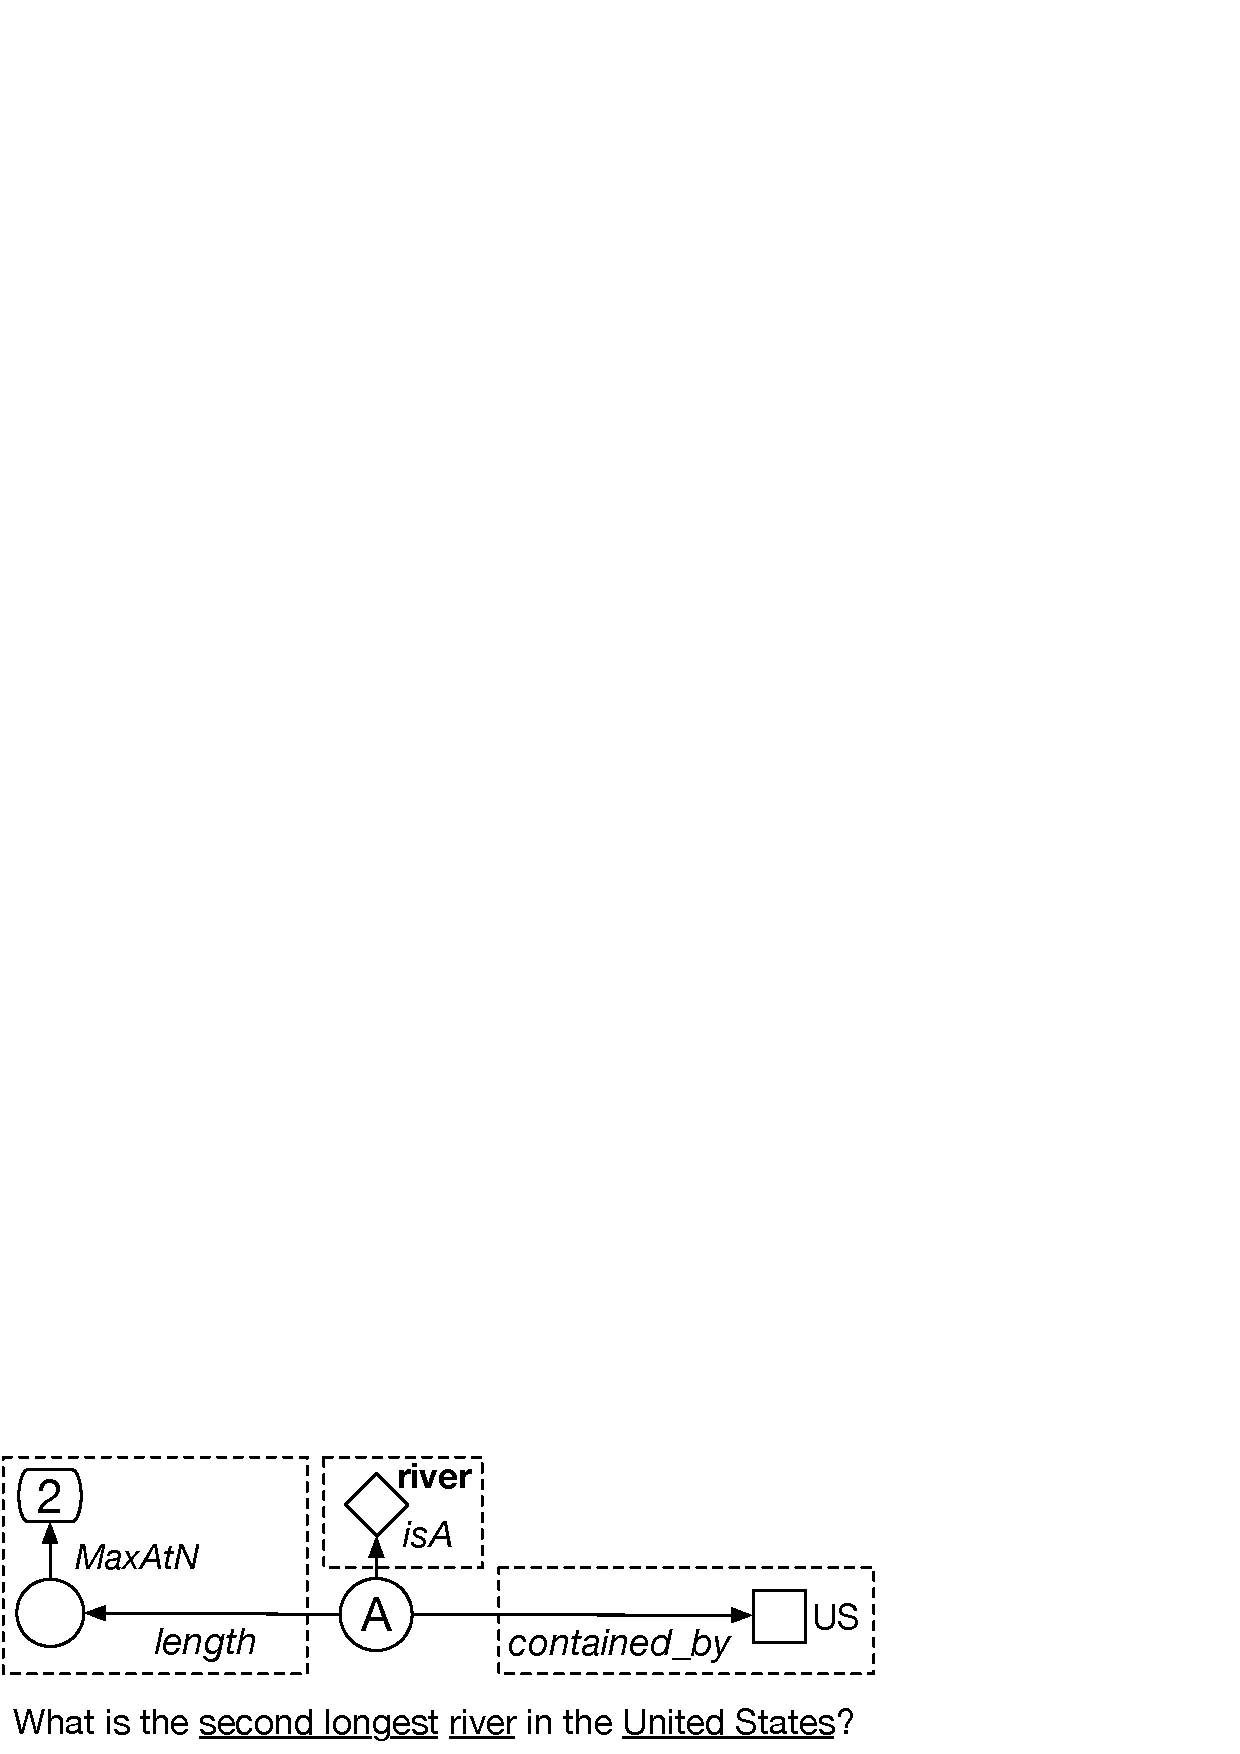
\includegraphics[angle=0]{figure/tabel/intro.pdf}}
\bicaption{Freebase缩略图。}
{A snapshot of Freebase.}
\label{fig:intro-freebase}
\end{figure}

由于上述知识库结构相似,研究方法具有普适性,
因此我们的工作主要基于资源最丰富的Freebase,
包含至少四千万个不同实体,三千种以上的常用类型,
六千种以上的常用谓词,以及十亿以上的事实三元组。
按功能划分,Freebase中的事实三元组可归为三类:
描述实体和类型间层次结构的
(实体, $IsA$, 类型)和少量(类型, $subTypeOf$, 类型)三元组;
描述实体间的关系的(实体, 关系, 实体)三元组;
描述实体自身属性的(实体, 属性, 属性值)三元组,
其中属性值为整数、浮点数、时间或字符串。
Freebase的一个缩略图如\figref{fig:intro-freebase}所示,
不同的实体、类型、谓词都有独立的编号,
例如谓词编号$type.object.type$代表$IsA$关系,$type.object.name$代表名称属性。
同时它们都具有唯一的名称属性值,部分实体还具有多个别名属性($common.topic.alias$)值。
例如实体\textit{m.02\_286}的名称为``New York City'' ,
具有别名``The Big Apple'' 、``Empire City'' 等;
谓词$location.location.contained\_by$名称为``Contained By'' ,描述了地点实体间的包含关系。
Freebase支持使用SPARQL语句进行结构化查询,
以类似SQL的语法从图结构知识库中筛选出满足查询条件的实体。
%SPARQL查询语句
%多元关系维护(例如FB使用Mediator)

%=====================%

%常见任务

%KB好比百科全书,而各种任务相当于,建立联系,例如QA:就像一个翻字典的人,理解的问句意义,在百科全书中找到对应的知识。

接下来,我们将关注在实体、关系、句子这三个递进层面上,
以知识库作为语义载体的一些自然语言理解问题。

%实体层面:实体链接
首先,实体层面的语义理解体现为实体链接任务,
即从自然语言文本中寻找出代表实体的短语,并匹配到知识库中的特定实体。
如同维基百科编辑者在页面中会添加一些超链接文本,
并指向其它实体页面,使得读者可以快速了解与当前页面相关的实体信息,
自动化的实体链接可以应用于开放领域的自然语言文本,
从而实现消歧义的目标。
文本输入可以是非结构化的文本,
也可以是半结构化形式,例如互联网中存在的表格。
\figref{fig:intro-wikification}展示了维基百科中关于赛车的一个页面,
其中纯文本和表格中的内容均被添加了超链接,指向了特定的车手、车队等实体页面。

\begin{figure}[th]
\centering
\includegraphics[width=0.95\columnwidth]{figure/intro/1_wikification.jpg}
%\scalebox{0.22}{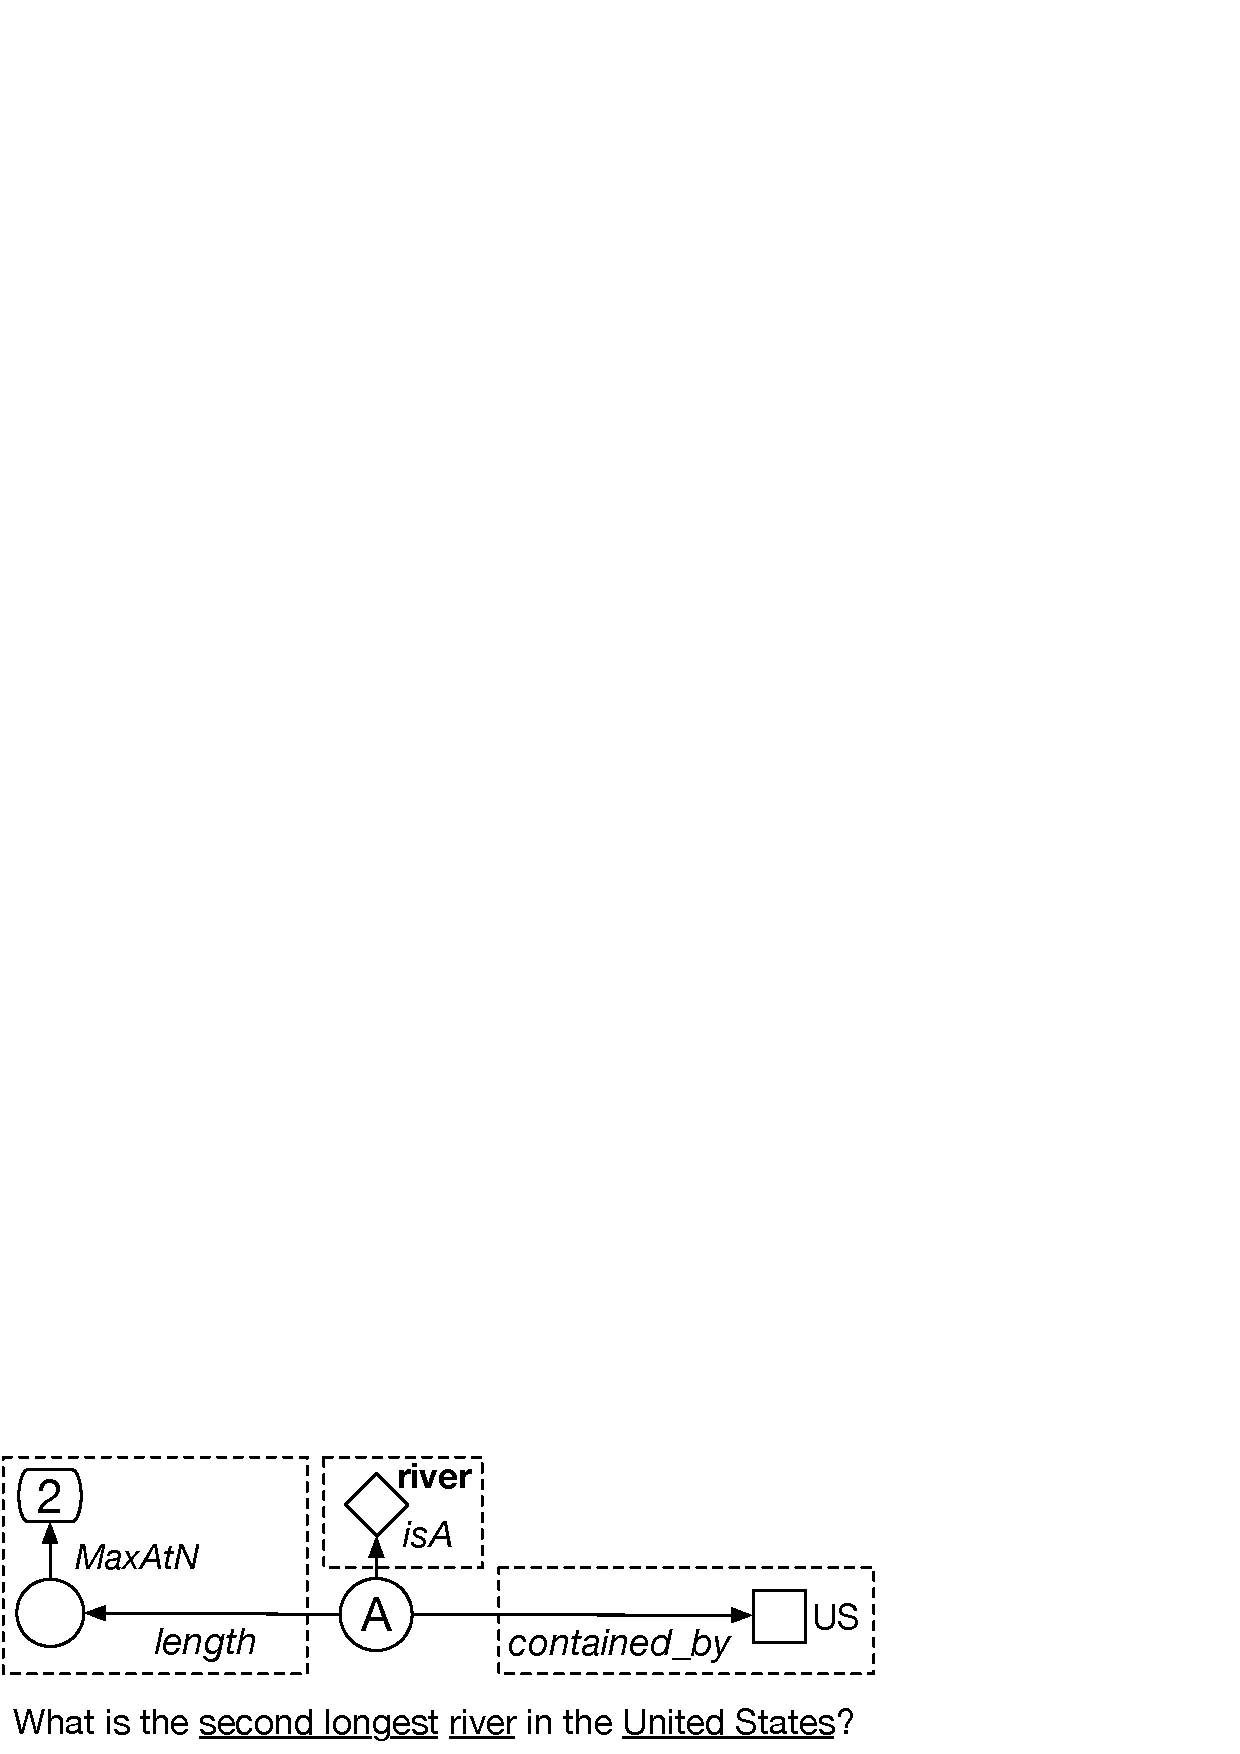
\includegraphics[angle=0]{figure/tabel/intro.pdf}}
\bicaption{维基百科中的实体与表格链接。}
{Entity and table linking in Wikipedia.}
\label{fig:intro-wikification}
\end{figure}

%实体链接的重点在于从多个候选中找出正确的那个实体,
%其本质为消除实体级别存在的一词多义性,
%例如短语``Michael Jordan''具有多个可能的候选,
%在维基百科中可能代表篮球明星、足球运动员、著名的机器学习教授,
%甚至更多不那么有名的人。
%在缺乏上下文信息的情况下,很难进行准确的链接。
%因此,一个良好的实体链接模型,相关性分数需要考虑多个因素,
%包括实体本身的先验知识,实体与短语的匹配程度,以及实体与短语所在上下文的契合度。


%关系层面:关系分类,知识库补全 

其次,对于关系层面的语义理解,   
一个传统任务为关系分类任务:
给定包含两个实体的句子,
将它们之间的关系归类至预定义的关系类别中。
%例如SemEval中的关系分类数据集
然而关系分类任务较难扩展到开放领域,
一方面,关系类别增多的同时,任务数据集的标注代价显著提升,
%SemEval-10, 19个类别
另一方面,不同于实体匹配,
知识库谓词和自然语言关系可能存在一定偏差,难以直接分类。
%由于知识库的构建 考虑了冗余性,
在这样的前提下,关系理解的实质在于,
如何利用知识库的已有谓词信息,学习目标关系语义。
这引出了知识库补全(Knowledge Base Completion)任务:
由于知识库中的事实可能存在缺失,
对于其中的目标谓词,能否推理出它和其它谓词之间的联系,
从而自动添加新的事实。
例如知识库中,某人的国籍缺失,那么可以根据其出生地所在的国家进行推测。
由于知识库中的事实三元组和自然语言的关系三元组具有类似形式,
因此目标谓词可以从知识库扩展到自然语言中。


最后,对于句子的语义理解,为了能充分利用知识库的信息,
我们关注描述客观事实的问句,通过自动问答任务衡量其语义理解能力。
自动问答具有广泛的应用场景,搜索引擎便是其中之一。
传统的搜索引擎工作方式依靠信息抽取相关算法,比较用户查询与网页的相似度,
主要利用词级别的共现模型,如TF-IDF\cite{leskovec2014mining},
或词级别的语义匹配模型,
如LSI\cite{deerwester1990indexing},pLSA\cite{hofmann1999probabilistic}等。
但对于用户输入的复杂问题,词级别的匹配难以直接定位到用户想要的答案或网页。
更加智能化的搜索引擎,则尝试对问题进行推理,并根据已有的知识库,
将答案定位至已知的实体中。
Google建立了以Freebase为基础的知识库(Google Knowledge Graph),
当用户搜索一些名词时,如\figref{fig:intro-se}中,用户搜索 ``george w bush'' ,
结果页面右侧会显示实体的信息框,包括其属性,以及与其关联的其它实体等。
而如\figref{fig:intro-qa}所示,当用户输入较为复杂的问题
``\textit{who was president of US when beijing olympics was held}'' ,
搜索引擎能在结果页面上方显示出自动回答的结果。
对比下方的传统页面搜索结果可见,
精确返回答案能大大提升查询过程的用户体验。

\begin{figure}[th]
\centering
\includegraphics[width=0.9\columnwidth]{figure/intro/3_sidebar.jpg}
%\scalebox{0.22}{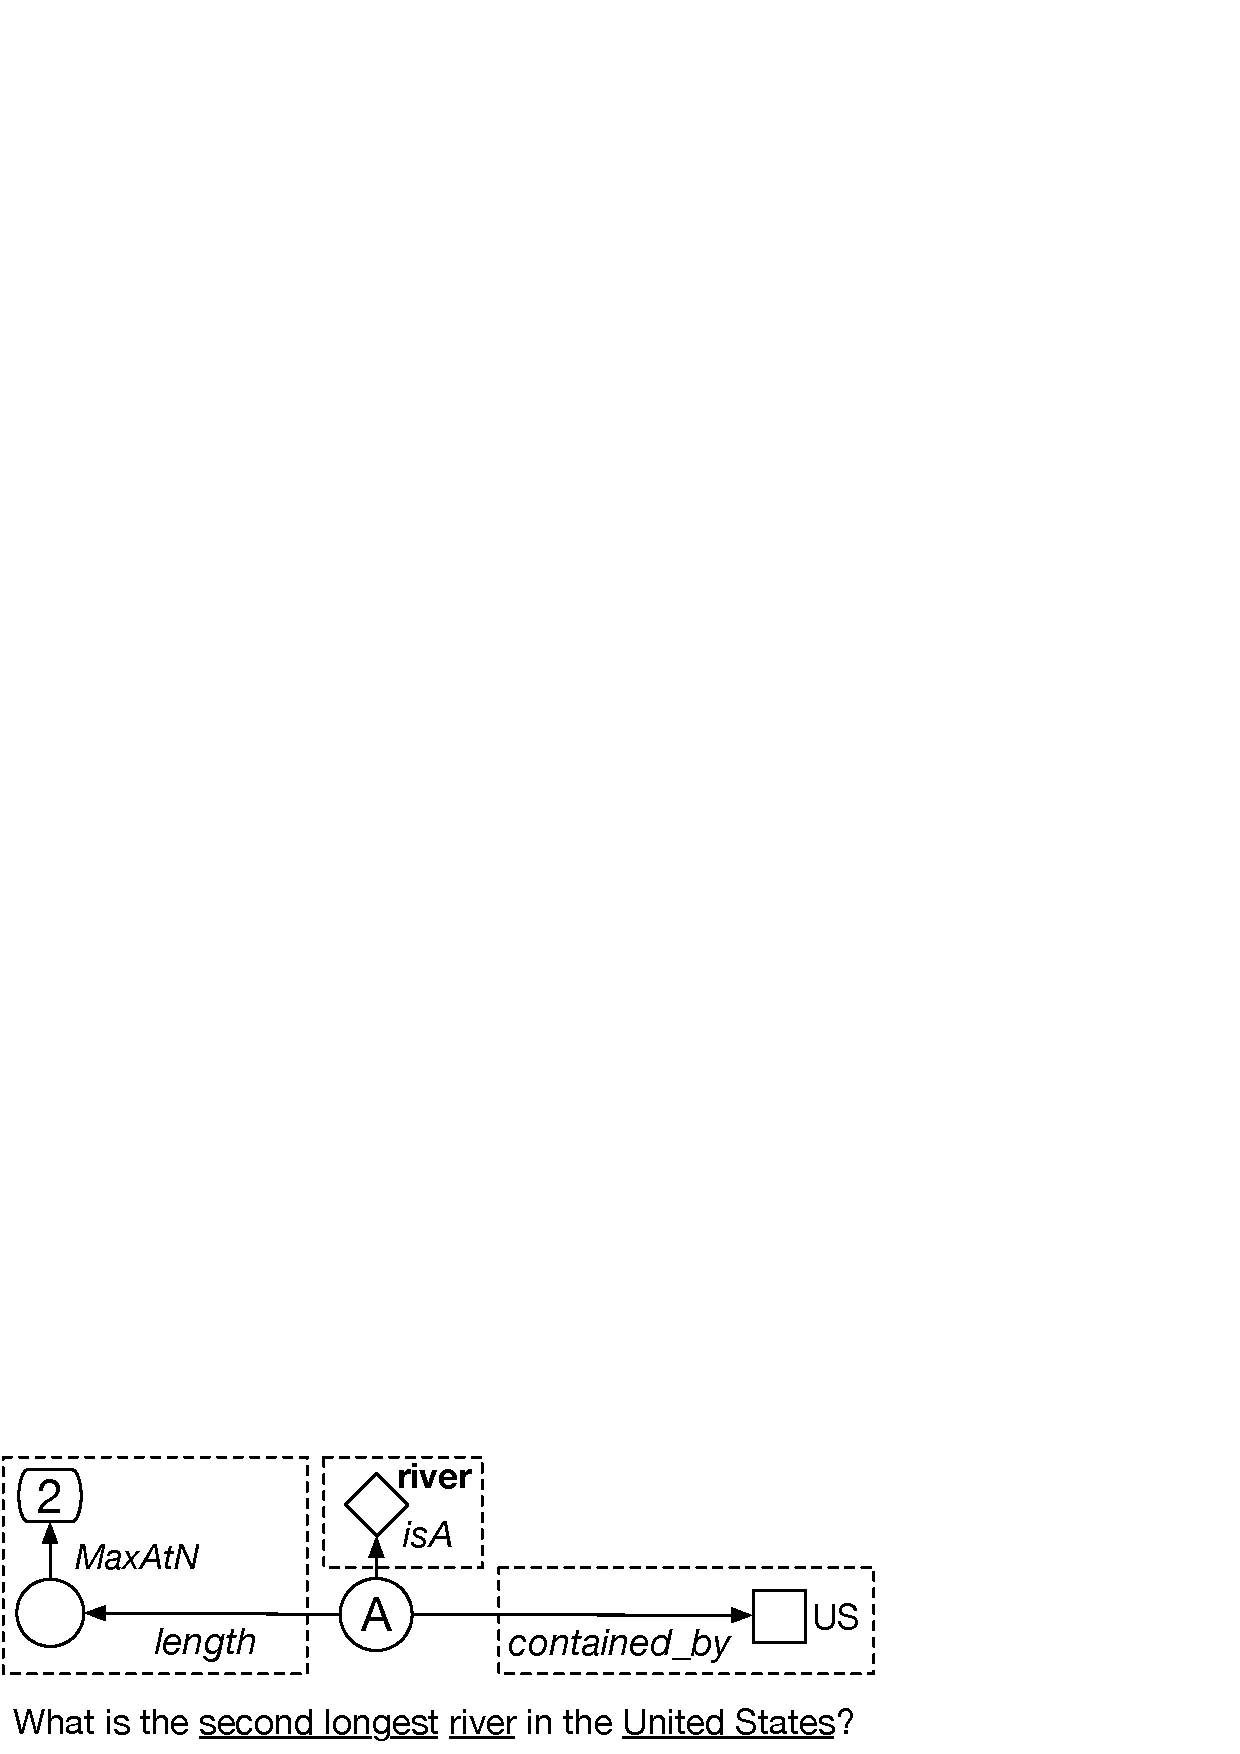
\includegraphics[angle=0]{figure/tabel/intro.pdf}}
\bicaption{搜索结果页面的右侧显示了当前实体的信息框。}
{The infobox at the right side of search result pages.}
\label{fig:intro-se}
\end{figure}

\begin{figure}[th]
\centering
\includegraphics[width=0.9\columnwidth]{figure/intro/3_search.jpg}
%\scalebox{0.22}{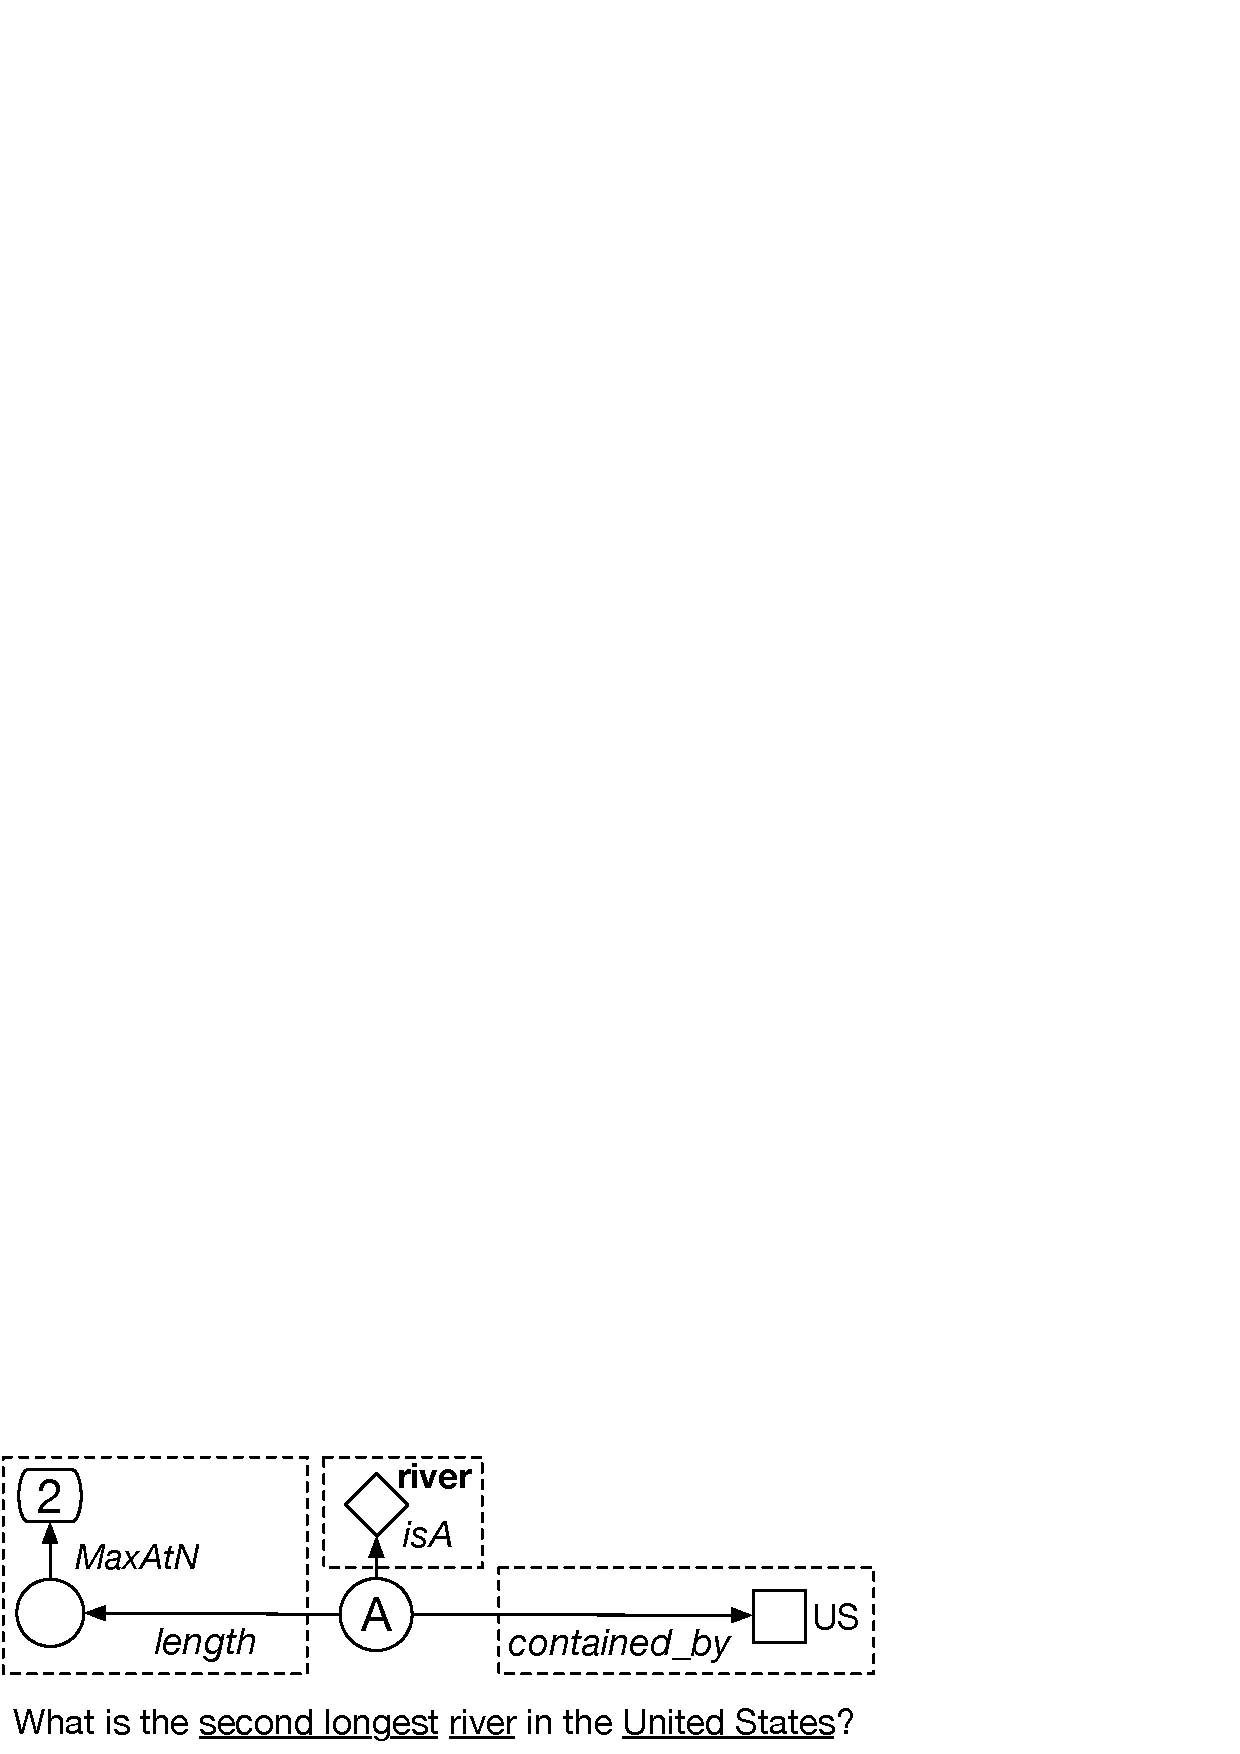
\includegraphics[angle=0]{figure/tabel/intro.pdf}}
\bicaption{搜索引擎精确返回复杂问题的答案。}
{The search engine precisely returns the answer of the complex question.}
\label{fig:intro-qa}
\end{figure}



% \begin{figure}[!htp]
%   \centering
%   \subcaptionbox{搜索引擎的右侧信息框\label{fig:intro-search:a}}
%     {\includegraphics[width=0.48\columnwidth]{figure/intro/3_sidebar.jpg}}
%   %\hspace{1em}
%   \subcaptionbox{搜索引擎精确返回问题答案\label{fig:intro-search:b}}
%     {\includegraphics[width=0.48\columnwidth]{figure/intro/3_search.jpg}}
%   \bicaption{搜索引擎的信息栏与自动问答。}
%             {Infobox and question answering in web search engines.}
%   \label{fig:intro-qa}
% \end{figure}

%3.问答系统
%基于知识库的自动问答 (客观事实类问题)
%对搜索引擎来说非常重要
%笨笨的引擎:基于IR,(TF-IDF,pLSA,LDA,embedding)抽象表达而已啦
%KG:基于语义理解,直接得出答案(右边栏)

实体、关系、问句的语义理解研究之间,存在着紧密的内在联系。
如\figref{fig:intro-relatedness}所示,一个具体的问句通常包括一至多个关系,
因此问句理解可以看做关系理解的扩展,
即在问句中寻找疑问词和多个已链接实体间存在的不同语义。
而作为自然语言理解的底层部分,实体理解是另外两者的基础,
它为关系理解提供了消歧义的三元组,也为问句理解划定了大致的语义范围,
由此可见,实体、关系、句子的语义理解具有级联关系,也是本文从这三个方向进行展开研究的动机。

\begin{figure}[th]
\centering
\includegraphics[width=0.9\columnwidth]{figure/intro/4_relatedness.eps}
%\scalebox{0.22}{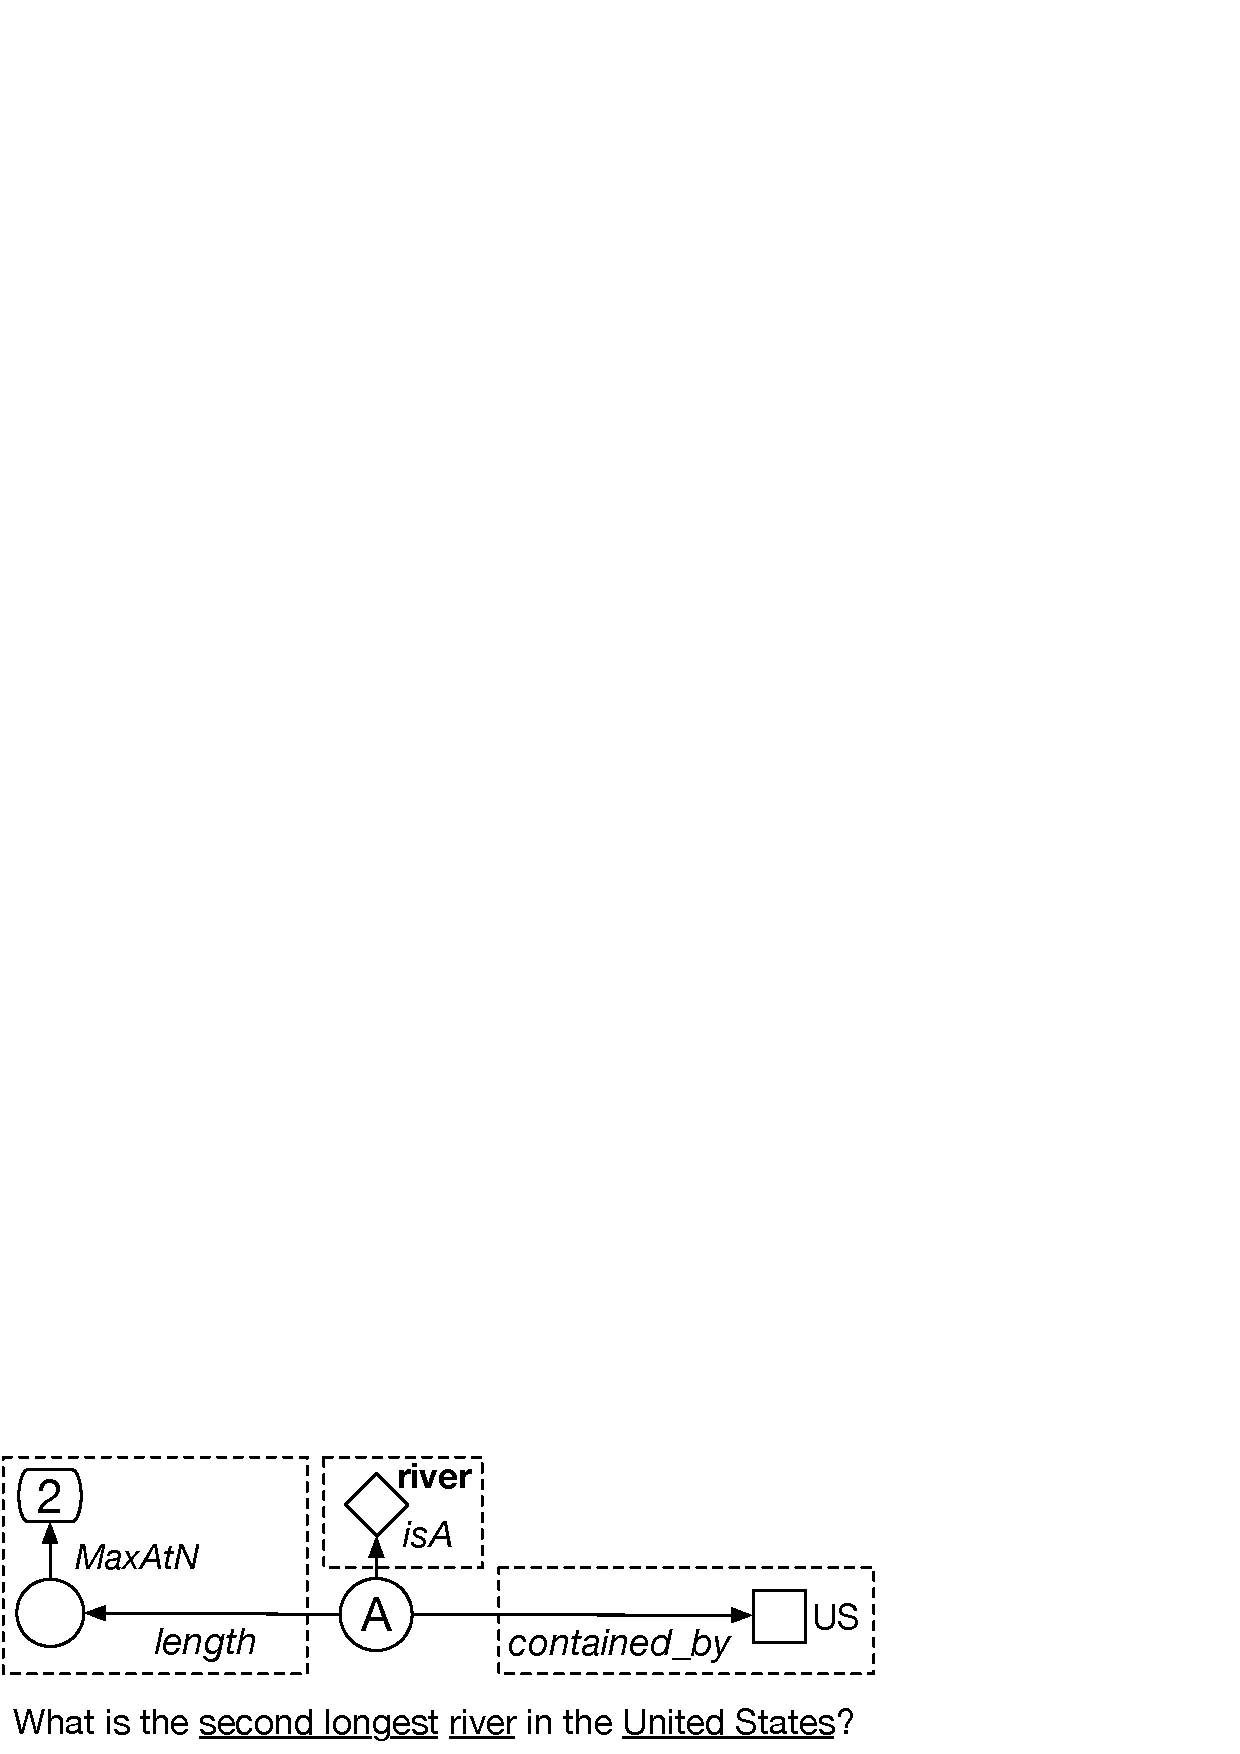
\includegraphics[angle=0]{figure/tabel/intro.pdf}}
\bicaption{实体、关系、句子语义理解之间的级联关系。}
{The cascaded relationship between entity, relation and sentence understanding.}
\label{fig:intro-relatedness}
\end{figure}


\section{研究现状}
%就是related work的精简版

上一节介绍了本文关心的语义理解问题,%接下来将简要介绍相关的研究现状。
本节中,我们延续实体、关系、问句语义理解这三部分,
回顾已有的一些相关工作。

实体链接的研究开始较早,Mihalcea等人\cite{mihalcea2007wikify}于2007年的研究
是以维基百科为载体进行链接的鼻祖工作。
对自然语言文本进行实体链接,主要分为两个步骤:
挖掘所有代表实体的短语,以及将短语映射至知识库中的特定实体。
短语挖掘可以通过字符串模糊匹配的方式进行收集,以保证较高的召回率。
之后的映射步骤则是实体链接模型的重点,
为了实现消歧义,需要利用短语所在文本的上下文特征,
以及多个短语所映射的实体之间的关联程度,
对于表格形式的文本输入,行列间实体所具有的特性也不可忽略。
根据以上观察,以特征工程为核心的机器学习模型被运用于此,
涵盖的特征主要包括基于维基内部超链接统计的先验概率,
基于TF-IDF模型\cite{guo2013link}的短语和实体的上下文相似度,
基于PMI\cite{ratinov2011local}、WLN\cite{shen2012linden}
等以维基共现频率衡量的不同实体间的相关度,
等等。
%特征工程模型具有较好 特征固然好,特征可扩展,但是耗费人力,同时新的特征可能并不适用与其它数据集。
考虑到特征设计耗费人力,且与特定任务高度相关,
更新的工作对基于深度学习的实体链接模型进行了研究,
模型依赖神经网络建立实体和短语上下文的特征表达,
并计算向量表达之间的相似度衡量短语和实体的匹配程度。
以文献\parencite{francis2016capturing}为代表,对于输入文本中的短语和维基百科中的实体,
模型可以关注不同粒度的上下文,利用卷积神经网络或循环神经网络对文本进行建模。
同时模型可以学习维基百科或知识库中,实体分类、类型等信息的向量表达,
以此丰富实体的语义特征,例如文献\parencite{sun2015modeling,gupta2017entity,nguyen2016joint}。
此外,若文本和知识库的语言不同,则为跨语言场景的实体链接。
通过翻译工具可以转化为单语言的实体链接,但受制于翻译步骤的准确率,
因此主要的模型使用了跨语言的词向量技术\parencite{ruder2017survey},
将不同语言下的单词映射至同一连续语义空间。


关系语义学习的研究,主要针对三元组级别,
给定目标关系或谓词,根据它所已知的三元组信息,对其语义进行建模。
按照关系语义的表示方法进行划分,
主要研究可以分为规则推导和知识库向量学习两类。
基于规则推导的模型中,
二元关系或谓词$p$等同于布尔函数$p(x, y)$,
对于给定目标,
模型旨在推导出由其它谓词构成的一阶逻辑表达式,%存在,任意,取反,等等
单个表达式的语义具有确定性,
同时人类可直接理解其语义表示,具有很高的可解释性。
早期研究以AMIE模型\cite{galarraga2013amie}为代表,挖掘具有高置信度的规则,
后续的改进研究着眼于挖掘多种可能的规则,并赋予不同权重或概率,
丰富语义表达能力,例如基于MLN模型的文献\parencite{jiang2012learning,zhang2012ontological},
以及生成负样本,对大量路径形式的规则进行特征学习的PRA模型\cite{lao2011random}
和SFE模型\cite{gardner2015efficient}。
另一个分支为知识库向量模型,
则依据已有的大量三元组信息,学习每一个实体和谓词的连续向量(或矩阵)表示,
并通过实体和谓词表示之间的代数运算,判断任意一个三元组事实的置信度。
具体置信度定义方式不同,ER-MLP模型\cite{dong2014knowledge}基于简单的多层神经网络;
RESCAL模型\cite{nickel2012factorizing}基于实体向量和谓词矩阵表示的双线性运算;
%HOLE模型\cite{nickel2015holographic}在RESCAL的基础上,
%使用向量循环平移技巧,大幅度降低谓语表示的维度;
TransE模型\cite{bordes2013translating}基于主谓宾向量之间的距离度量,
并衍生出一系列改进模型\parencite{wang2014knowledge,lin2015learning,xiao2016transg}。
这些方法能够更充分地利用海量三元组信息进行建模,
但是对谓词的语义缺乏直观解释。


对于问句理解与推理的研究,根据知识来源和答案形式的不同,可以分为两类任务:
基于结构化知识,答案通常为实体、数值等简单形式的知识库问答(KBQA);
以及基于非结构化文档,答案表示为自然语言文本片段的检索式问答(IRQA)。
后者不是我们的研究重点,现有的研究工作主要使用阅读理解模型
\parencite{chen2017reading,seo2016bidirectional},
从已有文档中抽取出最适合的文本片段作为答案。
与关系学习类似,根据对问句语义的表示形式,
解决知识库问答任务的方法也可分为两类。
%我们可以根据问句语义的表示形式
%类比于关系学习的两种方式,
%结构、非结构  划分为SP和E2E(信息抽取)。
第一类方法在相关文献\parencite{yao2014information,yao2015lean,dong2014knowledge,hao2017end}
中称为``{基于信息抽取的方法}''\footnote{该名称容易于检索式问答产生混淆,
这里讨论的是KBQA的一类方法,而不是IRQA。},
它们遵循端到端问答的思路:
%对问句进行实体链接,将知识库中和这些实体在一定距离内可达的其它实体作为候选答案,
对每个问句生成一定量候选答案后,
机器学习模型用来解决二分类问题,即判断每个\textless 问句,候选答案\textgreater 对是否正确。
%模型使用的特征来自 寻找问句和答案的直接相关,
模型使用的特征来自于候选实体在知识库中的信息
(包括名称,具有的类型,直接相连的谓词,相邻实体等)与问句中不同单词的交互,
早期模型使用特征工程,最新的研究则聚焦于利用神经网络进行特征表示学习。
%Yao等人的工作\parencite{yao2014information,yao2015lean}是这类方法的鼻祖,
%它通过分析答案在知识库中的邻接信息(包括其具有的类型,直接相连的谓语,相邻实体等),
%与问句特征进行交互,形成大量组合特征。
%深度学习在该方法中的代表文献\parencite{dong2014knowledge,hao2017end}
%旨在移除特征工程带来的劣势,
%这些模型主要使用卷积神经网络、循环神经网络以及注意力模块,
%用于学习问句语义在连续空间中的表示,
%同时根据候选答案在知识库的邻接信息,
%分别在类型、谓语等多个维度计算和问句的匹配程度。
这类模型的优点在于实现简单、训练数据容易获取,但缺点在于可解释性较差,
大量抽象特征的存在,使得人类难以理解某个候选答案被分类为正确或错误的根本原因。
%显然对于复杂的问题,能否准确找到周围的关键信息?
第二类方法称为语义解析(Semantic Parsing),
答案实体的选取依赖于对问句语义的结构化建模,
将其表示为知识库中的实体、类型、谓词组成的一阶逻辑表达式。
只需要将其转换为知识库上的结构化查询语言,例如SPARQL,
即可查询出所有满足语义的答案,因此具有很明确的可解释性。
%无差别答案
这类方法通常先根据问句信息,生成少量候选查询结构,
再利用机器学习算法训练问句和查询结构间的语义匹配模型,
因此整体效果取决于这两个步骤的质量。
查询结构生成方面,可依靠CCG\cite{cai2013large,kwiatkowski2013scaling}、
DCS\cite{berant2013semantic,berant2014semantic}等语法进行自底向上构建,
或者依赖深度优先搜索由简到繁生成查询结构\cite{yih2015semantic,bao2016constraint},
还可以基于固定模板进行生成\cite{cui2017kbqa,bast2015more},
以牺牲灵活性为代价,换取更有针对性的语义表达。
语义匹配计算方面,传统机器学习方法从候选结构的生成步骤中提取特征,
并与问句进行特征组合,以实现模型训练;
与此同时,深度学习方法通过学习知识库中不同实体、谓词等向量表示,
遵循``{编码—比较}'' 框架,将问句和查询结构的语义特征映射至同一空间,
并计算向量间的相似度。
基于深度学习的问答模型在近几年研究异常火热,
相关文献
\parencite{bordes2014open,bordes2015large,yin2016simple,yu2017improved,lukovnikov2017neural}等
在简单语义的问答场景中不断取得突破。
但对于更加复杂的问题,
这些模型并不能直接学习一个复杂查询结构的整体语义表达,
难以充分体现深度学习强大的特征表示能力。


%now 8.5 pages (basic: 5 pages)

\section{主要工作和贡献}

%三个部分分别展开
%每个部分先讲研究目标内容(就是我们想尝试解决的薄弱问题)
%再讲我们的方法
本节中,我们具体介绍本文的主要工作,包括实体、关系、问句理解三方面的研究内容,
技术难点,以及我们我们的贡献。


\subsection{实体理解问题}

对于实体的理解,我们聚焦于跨语言场景下的表格实体链接任务,
即以非英文编写的表格作为输入,将每个单元格对应的实体链接至英文知识库。
我们以该任务作为研究对象,主要有两个动机:
首先,英文知识库规模最为庞大而全面,%同时英文也是连接不同语言的重要纽带,
有助于让不同语言的人类共同理解知识;
其次,表格行列间通常存在着特定的关系,因此相比纯文本中的实体链接,
表格链接能更有效地帮助知识库进行知识扩充。
%目前学术界缺乏对该任务的研究,本文是首次
本文是学术界首次对该任务进行具体研究,
具有以下两个主要特点:
1) 短语和目标实体处于不同语言中,必须在字面相似之外,寻找候选实体收集和匹配度量的方式;
2) 每个单元格和目标实体间的匹配可以体现在多个粒度,例如单元格自身,以及其所在的行列上下文,
同行列的实体之间还存在明显的关联性。
%带来了新的挑战。

为了解决跨语言表格链接问题,我们提出了基于神经网络和跨语言词向量的链接模型。
该模型首先通过已有翻译工具进行候选实体的收集,但匹配过程并不依赖唯一的翻译结果;
其次,模型利用多语言词向量的训练,将不同语言中的实体和短语映射至相同维度空间,
实现最基本的匹配度量;
%并结合已有词表完成更好的映射
再次,模型利用深度神经网络学习表格与目标实体间不同粒度的匹配特征,
并提出了基于方差计算的一致性特征,以捕捉同列实体所具有的同质性;
最后,模型基于联合训练思路,以优化整张表格的匹配程度作为目标,
进一步提升整体链接质量。
在跨语言和单语言两个场景上的实验表明,
我们的模型有效捕捉表格中实体之间的特殊联系,同时在跨语言场景中具有稳定而良好的效果。

\subsection{关系理解问题}

对于关系的理解,我们旨在利用知识库构建人类可理解的结构化表达,
以描述二元关系语义,并用于下游任务中,例如关系分类和知识库补全。
对关系的建模问题,有以下两个特点:
1) 与实体类似,自然语言中关系存在着多义性,即对应多种描述方式;
2) 自然语言关系和知识库谓词存在语义间隔,由于知识库的构建避免了信息冗余,
一个关系未必能直接映射到知识库中的单个谓词。

为了学习关系的语义,我们根据开放式信息抽取系统在海量文本中
抓取的结果为输入,获取单个关系的多个主谓宾三元组,
从而以数据驱动的方式进行语义建模,并由粗细两个粒度进行分析。
在粗粒度方向,我们关注于关系的多义性,
并通过其主宾语的类型搭配来区分其不同的语义。
为此,我们对知识库中不同类型间的包含关系进行挖掘,
构建出更加丰富的类型层次结构,并根据主宾语类型对的覆盖率和精细度进行筛选,
生成最能够代表关系语义的类型搭配。
实验结果表明我们的模型效果优于传统的选择偏好模型。
在细粒度的方向,我们关注关系语义的精确表达,
使用人类能理解的图结构作为语义的表达形式。
我们提出了基于规则推导的模式图推理模型,
该模型从已有的关系三元组出发,用知识库中的谓词序列连接主宾语,
并在此基础上搜索额外的限制,生成一系列具有 ``{路径+分支}'' 形式的复杂模式图。
随后,模型再次利用已有实例,学习候选模式图上的概率分布,
在描述关系多义性的同时,也完成了具体和宽泛模式图之间的平衡。
我们将生成的模式图概率分布运用于知识库补全任务中,
实验结果显示,我们的模式图推理模型不仅具有高度可解释性,
而且效果优于其它规则推导模型和新兴的知识库向量模型,

\subsection{问句理解问题}

对于问句的理解,我们着眼于基于知识库的自动问答任务,
即对描述客观事实的问句,从知识库中寻找出其对应的一个或多个答案实体。
对于只包含简单语义的问题,自动问答的过程等价于将问题转换为
知识库上的一个事实三元组。
然而,人类提出的问题并不总以简单形式呈现,而是会在其中加入更多限制。
例如问句中存在多个与答案相关的实体、类型,或是包含时间、顺序信息等,
对应着多条和目标答案相关的三元组,因此面向简单问句的模型便不再奏效。
在复杂语义场景中,知识库问答具有以下挑战:
1) 如何从问句中发现存在的多个关系,并组合成为一个候选语义结构;
2) 如何计算自然语言问句和复杂语义结构之间的匹配程度。

我们提出了针对复杂问句的的深度学习语义匹配模型。
该模型的思路是细粒度关系理解模型的延续,
使用知识库中的实体、谓词、类型等信息作为基本元素组成图结构,
称其为查询图,用于表示问句语义。
它在具有良好可解释性的同时,
可以通过结构化查询语句(如SPARQL)在知识库中找出所有满足语义的答案实体。
模型首先利用多阶段候选生成方式,由简到繁生成不同的候选查询图,
我们已有工作进行优化,更快速和准确地表示类型和时间限制。
之后,语义匹配模型的核心是利用深度神经网络学习问句和查询图整体的匹配程度,
我们的创新点在于对复杂的查询图进行整体编码,生成其唯一的向量表示,
从而捕捉问句中不同语义成分的组合特征。
同时,我们利用依存语法分析作为对问句字面信息的补充,
使模型能更有效地将问句和不同的语义成分对齐。
实验结果表明,基于复杂查询图的深度学习模型
在多个复杂问题和简单问题数据集上都具有良好的性能。



\section{论文结构}

本文组织结构如下:

第一章主要介绍了知识库的发展,以及语义理解的研究背景,并从实体、关系、问句三个角度出发,
对研究现状进行概述,最后介绍了本文在这三个方面的语义理解的研究内容和贡献。

第二章主要对实体、关系、问句的语义理解问题进行综述,
围绕具体任务介绍这些问题的基础知识,以及已有的相关工作。

第三章围绕实体理解问题,主要介绍本文在跨语言场景中,面向表格文本进行实体链接的深度学习模型。

第四章围绕关系理解问题,主要介绍本文对自然语言关系的粗粒度和细粒度建模,
前者面向关系的多义性,后者面向关系的准确语义表达,并运用于知识库补全任务。

第五章围绕问句理解问题,主要介绍本文在知识库问答任务中,面向复杂问句的深度语义匹配模型。
%第五章,针对复杂问题设计的系统,在多个数据集上可以得到优秀的结果。(分复杂和简单来聊)

第六章主要对论文工作进行总结,并展望未来可以继续的研究工作。

